% mnras_template.tex
%
% LaTeX template for creating an MNRAS paper
%
% v3.0 released 14 May 2015
% (version numbers match those of mnras.cls)
%
% Copyright (C) Royal Astronomical Society 2015
% Authors:
% Keith T. Smith (Royal Astronomical Society)

% Change log
%
% v3.0 May 2015
%    Renamed to match the new package name
%    Version number matches mnras.cls
%    A few minor tweaks to wording
% v1.0 September 2013
%    Beta testing only - never publicly released
%    First version: a simple (ish) template for creating an MNRAS paper

%%%%%%%%%%%%%%%%%%%%%%%%%%%%%%%%%%%%%%%%%%%%%%%%%%
% Basic setup. Most papers should leave these options alone.
\documentclass[fleqn,usenatbib]{mnras}

%%% DEBUG SETTINGS - remove at the end %%%%%%%%%%%%%%%
\usepackage{silence} % silence error warinings
\WarningFilter{caption}{Unsupported document class} % caption doesn't know mnras..
\hbadness = 5000
\vbadness = 10000
\usepackage{}

% MNRAS is set in Times font. If you don't have this installed (most LaTeX
% installations will be fine) or prefer the old Computer Modern fonts, comment
% out the following line
%\usepackage{newtxtext,newtxmath} % not yet supported on arxiv and uni computer
%\usepackage{txfonts}

% Depending on your LaTeX fonts installation, you might get better results with one of these:
%\usepackage{mathptmx}
%\usepackage{txfonts}

% Use vector fonts, so it zooms properly in on-screen viewing software
% Don't change these lines unless you know what you are doing
\usepackage[T1]{fontenc} % make sure font is supported
% \usepackage{ae,aecompl} %obsolete when using modern fonts
\usepackage[final]{microtype} % make sure font is supported
% and a suitable font
\usepackage{lmodern} % use a modern font with T1 support
%\usepackage{cm-super} % use a modern font with T1 support


%%%%% AUTHORS - PLACE YOUR OWN PACKAGES HERE %%%%%

% Only include extra packages if you really need them. Common packages are:
%\usepackage[dvipdfmx]{graphicx}	% Including figure files
\usepackage{graphicx} % Including figure files
\usepackage[skip=0pt]{subcaption}
\usepackage{amsmath}	% Advanced maths commands
\usepackage{amssymb}	% Extra maths symbols
%\usepackage{bmpsize}  % PS still needs this for correct bounding boxes?

% TODO stuff, comment out for final submit
\usepackage{todonotes} % as long as we are editing...
\usepackage{showframe} % for debug
\overfullrule=5pt      % show overfull boxes

% I disabled hyperlink in the cls und included it here because of bugs
\usepackage{hyperref}   % Hyperlinks
\hypersetup{colorlinks=true,linkcolor=blue,citecolor=blue,filecolor=blue,urlcolor=blue}

%%%%%%%%%%%%%%%%%%%%%%%%%%%%%%%%%%%%%%%%%%%%%%%%%%

%%%%% AUTHORS - PLACE YOUR OWN COMMANDS HERE %%%%%

% Please keep new commands to a minimum, and use \newcommand not \def to avoid
% overwriting existing commands. Example:
%\newcommand{\pcm}{\,cm$^{-2}$}	% per cm-squared


\newcommand{\inclfig}[2]{
  \centering
  \begin{subfigure}{0.5\linewidth}
    \includegraphics[width=\linewidth]{spaghetti/#2_input}
  \end{subfigure}%
  \begin{subfigure}{0.5\linewidth}
    \includegraphics[width=\linewidth]{spaghetti/#2_img1}
  \end{subfigure}%
  \\[-1px]%
  \begin{subfigure}{0.5\linewidth}
    \includegraphics[width=\linewidth]{spaghetti/#2_img3_ipol}
  \end{subfigure}%
  \begin{subfigure}{0.5\linewidth}
    \includegraphics[width=\linewidth]{spaghetti/#2_img2}
  \end{subfigure}%
  \\[-1px]%
  \begin{subfigure}[b]{\linewidth}
    \includegraphics[width=\linewidth]{masses/#1_#2_mstel_vs_mtot}
  \end{subfigure}
}

\newcommand{\lenstitle}[1]{\noindent\textbf{#1} --}
\newcommand{\params}[3]{(\(\Theta_\text{E}:#1\), $\varepsilon:#2$, $\alpha_\varepsilon:#3$ )}


\newcommand{\asw}[1]{ASW000#1}
\newcommand{\sw}[1]{SW~#1}
\newcommand{\model}[1]{SL model~#1}

\newcommand{\figref}[1]{Figure \ref{fig:#1}}
\newcommand{\Figref}[1]{Figure \ref{fig:#1}}

%%%%%%%%%%%%%%%%%%%%%%%%%%%%%%%%%%%%%%%%%%%%%%%%%%

%%%%%%%%%%%%%%%%%%% TITLE PAGE %%%%%%%%%%%%%%%%%%%

% Title of the paper, and the short title which is used in the headers.
% Keep the title short and informative.
\title[Short title, max. 45 characters]{Preliminary categorisation of SpaceWarps candidates}

% The list of authors, and the short list which is used in the headers.
% If you need two or more lines of authors, add an extra line using \newauthor
\author[R. Kueng et al.]{
Rafael Kueng,$^{1}$\thanks{E-mail: rafael.kueng@uzh.ch}
Presenjit Saha,$^{1}$
Lucy Oswald$^{3}$
%and Fourth Author$^{4}$
\\
% List of institutions
$^{1}$Physik Institut, University of Zurich, Winterthurerstrasse XXX, Zurich 8057, Switzerland\\
$^{2}$Department, Institution, Street Address, City Postal Code, Country\\
$^{3}$Another Department, Different Institution, Street Address, City Postal Code, Country
%$^{4}$Another Department, Different Institution, Street Address, City Postal Code, Country
}

% These dates will be filled out by the publisher
\date{Accepted XXX. Received YYY; in original form ZZZ}

% Enter the current year, for the copyright statements etc.
\pubyear{2016}



% Don't change these lines
\begin{document}
\label{firstpage}
\pagerange{\pageref{firstpage}--\pageref{lastpage}}
\maketitle

% Abstract of the paper
\begin{abstract}
This is a simple template for authors to write new MNRAS papers.
The abstract should briefly describe the aims, methods, and main results of the paper.
It should be a single paragraph not more than 250 words (200 words for Letters).
No references should appear in the abstract.
\end{abstract}

% Select between one and six entries from the list of approved keywords.
% Don't make up new ones.
\begin{keywords}
keyword1 -- keyword2 -- keyword3
\end{keywords}

%%%%%%%%%%%%%%%%%%%%%%%%%%%%%%%%%%%%%%%%%%%%%%%%%%
%%%%%%%%%%%%%%%%% BODY OF PAPER %%%%%%%%%%%%%%%%%%
%%%%%%%%%%%%%%%%%%%%%%%%%%%%%%%%%%%%%%%%%%%%%%%%%%

\section{Introduction}

Here we cite \cite{2015MNRAS.447.2170K}.

\section{Methods}

\subsection{Parameterisation of pixel models} \label{sec:parameter}
In order to fit the set of pixelated models to a single parameterised model, a program was written that took a parameterised function and subtracted from it the mean and the principle components of the data, which were calculated using classical Principle Component Analysis.
This created the residuals function.
The number of components defined as principle was varied to test how this affected the output, and it was found that using 5 principle components tended to give a reasonable approximation.
A masking function was added which selected only the data points that fell inside the image of the lens, and the principal components were clipped in order to keep the values inside the region of the ensemble of models.
Any value higher than the clip was set to be the clip value.
This was chosen to be 2.5 as, assuming that the data follows a Gaussian error distribution, almost all the values for the variance should lie between 2 and 3 standard deviations from the mean.
Minimising the residuals function produces the set of parameters that fit the parameterised function to the original pixelated ensemble most closely.
A least squares fit was used to perform this minimisation.


The parameterised model function was obtained from the gravitational potential of an isothermal ellipsoid mass distribution \cite{2001astro.ph..2340K}.
This model is frequently used to describe gravitational lenses as it tends to fit well with observations.
The isothermal ellipsoid model outputs three useful parameters: the radius of the Einstein ring, the ellipticity of the model and the angle of the ellipticity from the vertical, giving the orientation of the galaxy.
By applying this model to simulated lenses for which the values of these parameters were already known, it was possible to gain an estimate of the projected accuracy of the results, before applying the model to the candidate lensing galaxies.


\subsection{HiRes / Subsampling of central region}
In a previous paper \cite{2015MNRAS.447.2170K} we identified the problem of the tendency of the models to be too shallow.
We pinned down the problem to the central region and are confident to have it fixed with enabling sub pixel sampling in the central area.
The software allows for subsampling parameters of radius of pixels $r_\text{subs}$ and amount of subpixels per pixel $n_\text{subs}$.
\Figref{subsampling} shows the results of different settings for $r_\text{subs}$ and $n_\text{subs}$.
We can see that even the computationally least expensive settings of $r_\text{subs}=1$ and $n_\text{subs}=3$ leads to drastically improved profiles.

\begin{figure}
  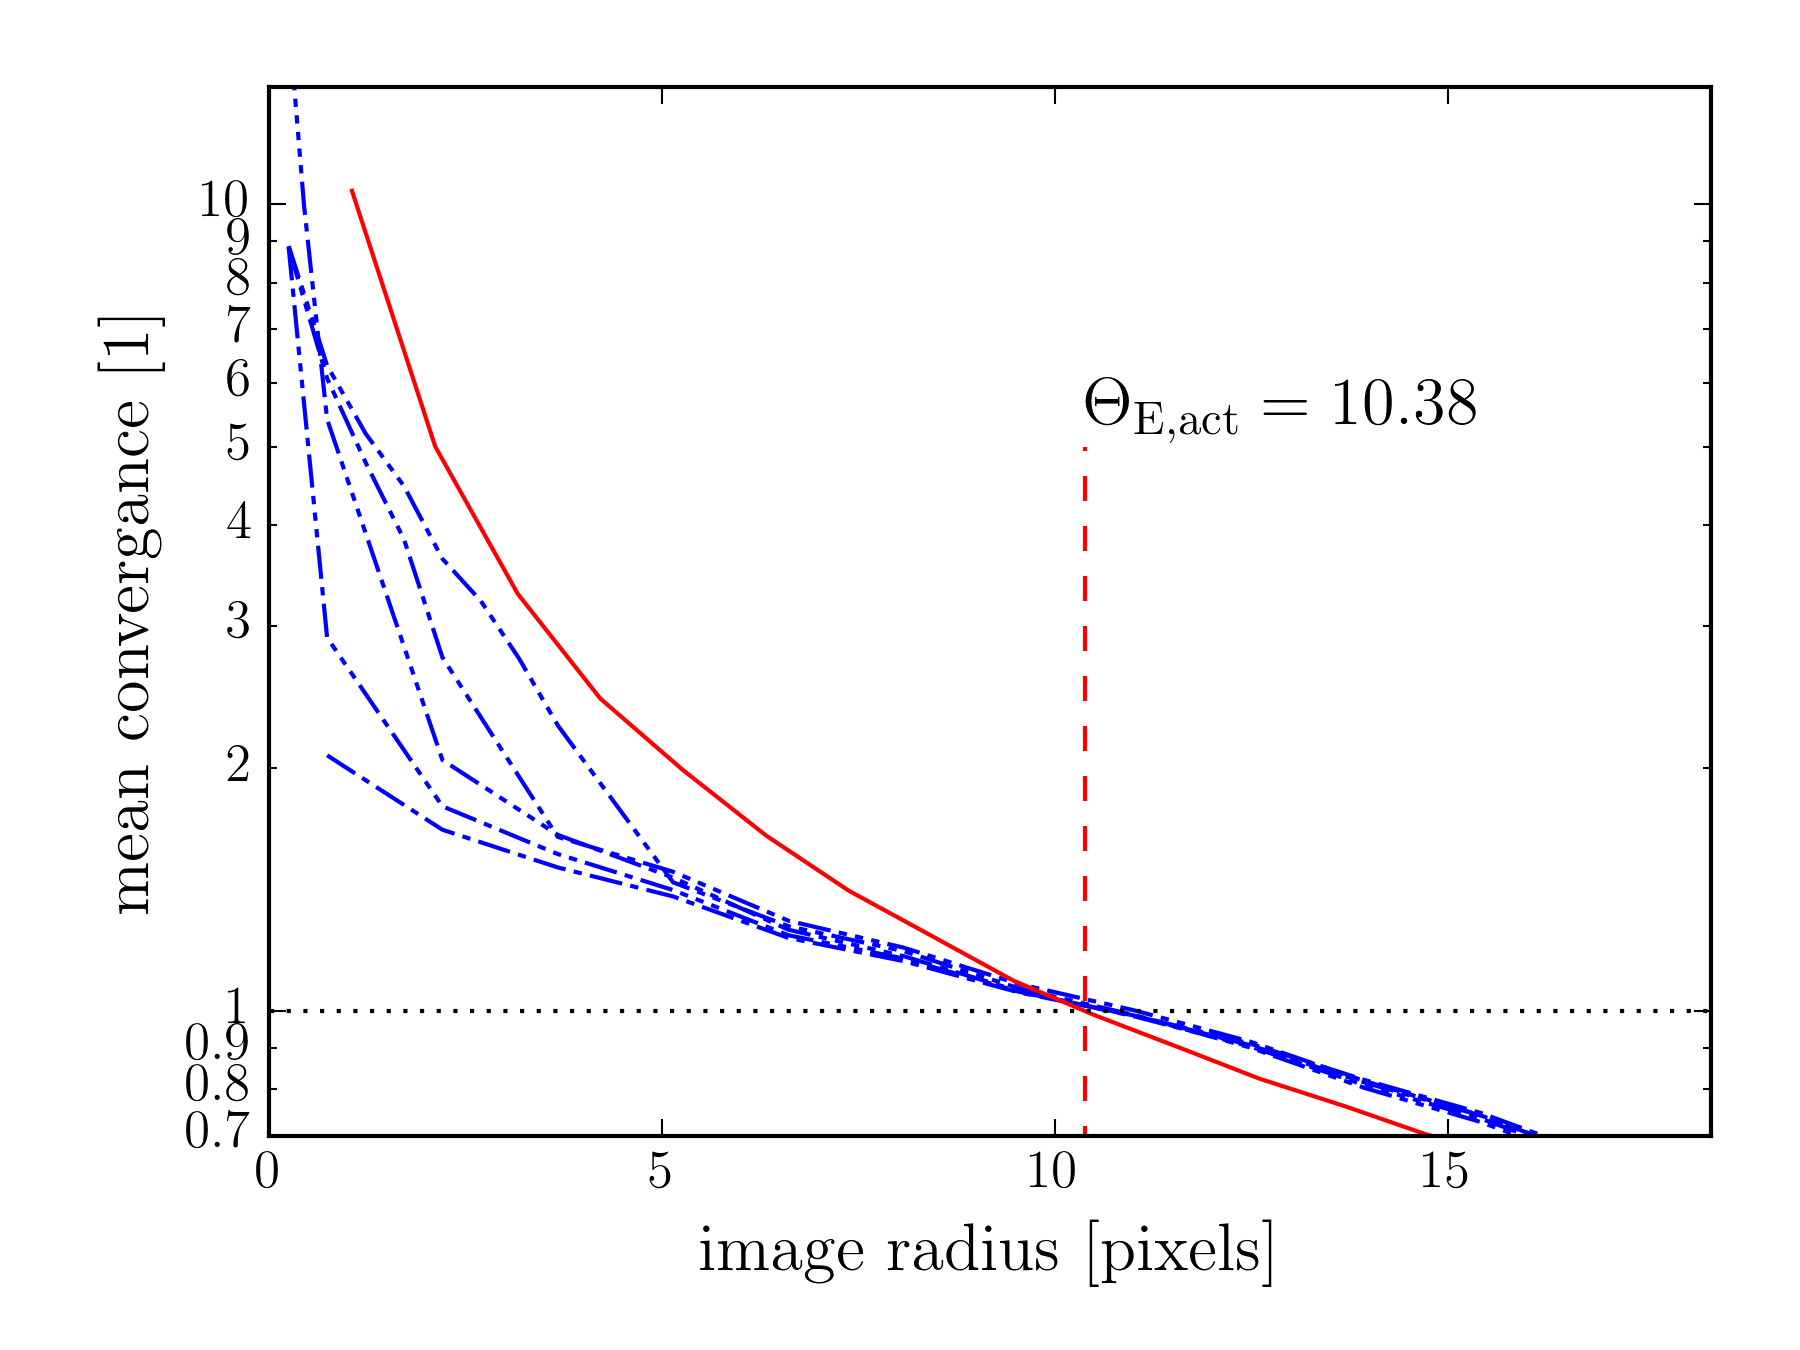
\includegraphics[width=\linewidth]{hires/007022_kappa_encl}
  \caption{
    Circularly averaged mass profile for different subsampling of central region.
    Red line without subsampling, blue lines show subsampling with dash-dot pattern showing the mode.
    $\cdot / \cdot \cdot \cdot$: $r_\text{subs}=1$ inner pixels, each subdivided into $n_\text{subs}=3$ sub pixels.
    $\cdot / \cdot \cdot \cdot \cdot \cdot$: $r_\text{subs}=1$, $n_\text{subs}=5$.
    $\cdot \cdot / \cdot \cdot \cdot $: $r_\text{subs}=2$, $n_\text{subs}=3$.
    $\cdot \cdot \cdot / \cdot \cdot \cdot $: $r_\text{subs}=3$, $n_\text{subs}=3$.
    }
  \label{fig:subsampling}
\end{figure}




\subsection{Additional / Improved Synthetic Image}

Volunteers often ask about better indicators to identify wether the modelling resulted in a ``good'' or ``bad'' model.
We developped a prototype of a better syntetic image than just the rendering of a \todo{insert currently used source profile} profile.
It operates on the composite input image.
The user has to mask the supposed lensed images.
The algorith then establishes a grid on the source plane and projects the masked pixels of the lense plane back to the source plane.
Multiple lens plane pixels fall onto one source plane pixel and get averaged.
The new synthetic image then reverses the mapping, coloring each pixel in the lens plane with the corresponding values of the source plane pixel.

\begin{figure}
  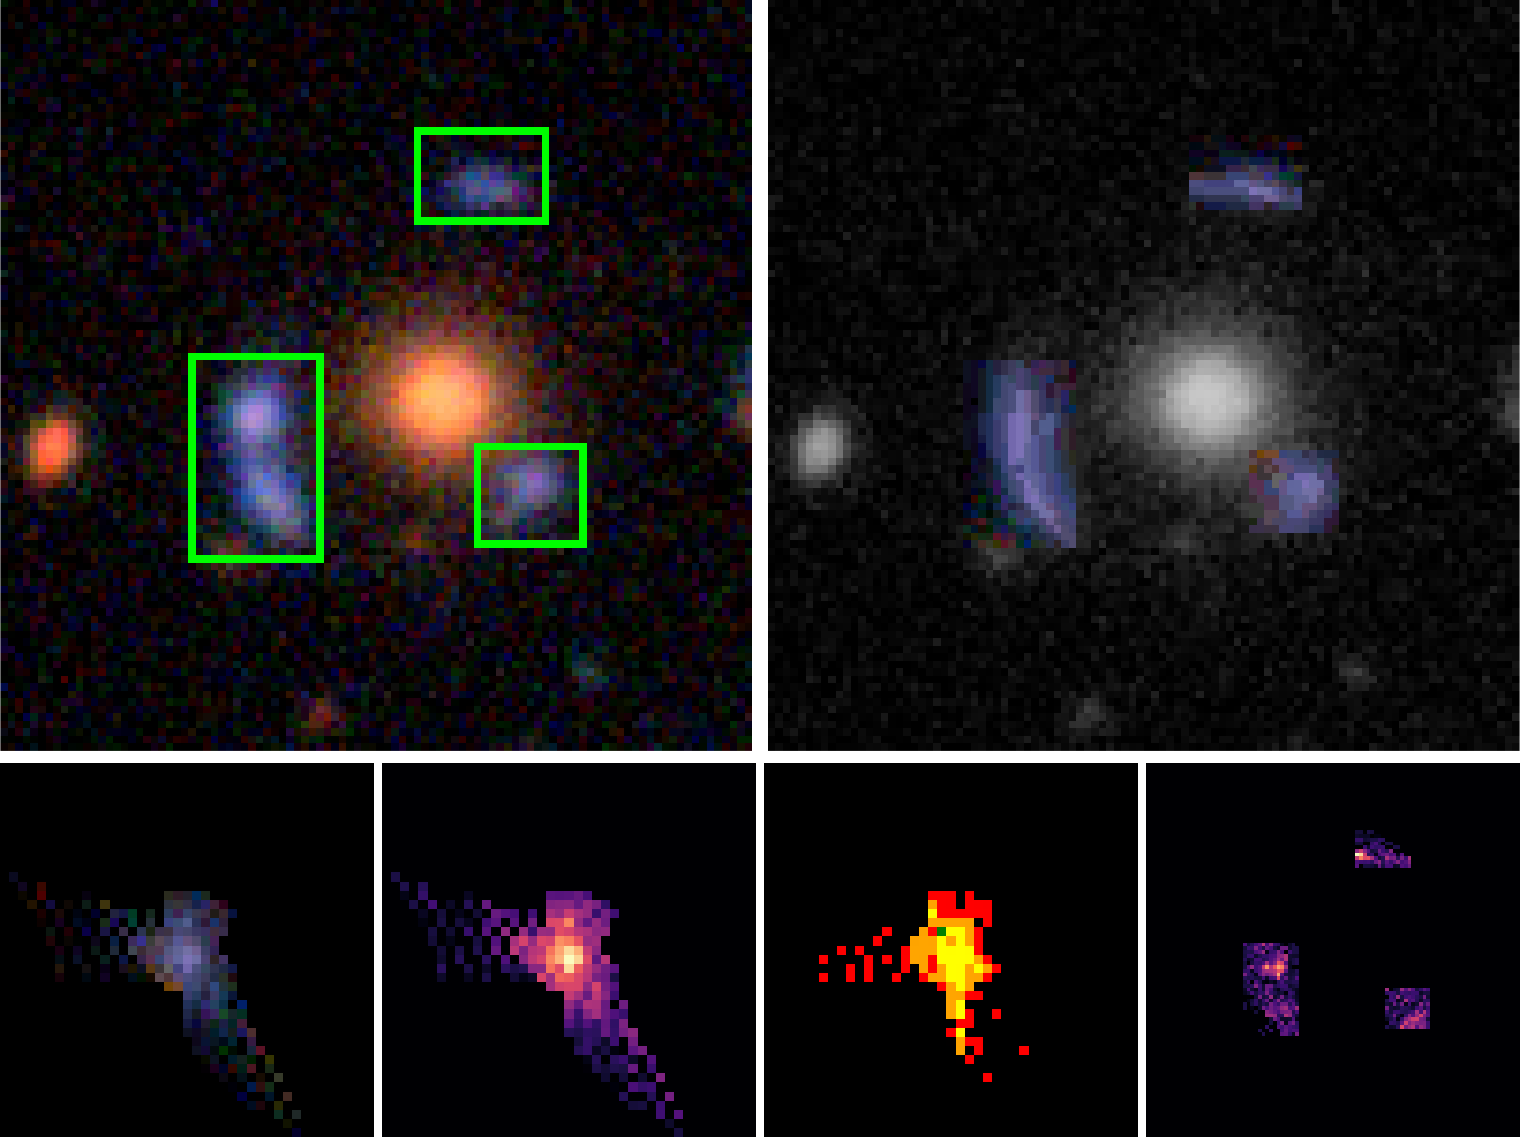
\includegraphics[width=\linewidth]{img/new_synth_img_detailed}
  \caption{
      Top-left: Orginal image, top-right: improved synthetic image for candidate \sw{5} (\asw{7k4r}) and model \model{12402};
      bottom from left to right:
        reconstructed source in color,
        intensity (grayscale),
        count of lens plane pixels per source plane pixel,
        residual of orginal image to improved syntetic image in grayscale
    }
  \label{fig:synthimg}
\end{figure}






\section{Results}
Throu visual inspection of the most popular models generated for each candidate and data generated by those models we classified the candidates in four categories.
The data available is shown in \figref{SW58}.
\todo{better explain criterias?}
The following sections list all the models for all the categories, each with a short explanation of the reasons.
Additionally, selected models are presented in figures for demonstration.

% 
% \subsection{Spectra}
% Candidates to follow up with a spectral analysis. 
% 
% 
% \subsection{Bad models}
% Candidates that need more work to be modelled.
% Or that have features that are hard / impossible to model with the current SpaghettiLens version.
% Examples are group lenses
% 
% 
% 
% \subsection{Non Lenses}
% Those are most probly non lenses, 



\subsection{plausible}

The plausible candidates fail in one category, but are quite convincing in all the others.
One particular reason for a candidate to end up in this category is that is has extended arcs, what is hard to modell with the current version of the program.
Thats why we recomend them for a following up study, for example for taking spectras or other follow up obersatories and for other modelling programs for a try.


\lenstitle{SW01 (ASW0004dv8)}
  This is some text that says something more than this line.

\lenstitle{SW08 (ASW00099ed)}
  Simple lens with two images;
  model has minor arthefacts.

\lenstitle{SW11 (ASW0002qtn)}
  Simple small arc;
  model nedes minor refinement;
  quite low mass ratio
  
\lenstitle{SW12 (ASW0003wsu)} 
  faint arc, bright overall situation, no counter image;
  has good model;
  low Mstel and low Mlens
  
\lenstitle{SW21 (ASW0004m3x)} 
  clear arc, no counter image; inbetween two external sources;
  model needs work, predicts additional images. play with external mass / sheer?
  Mass ratio low.
  
\lenstitle{SW27 (ASW0006jh5)} 
  (really plausible?)
  unclear situation, but arc is visible;
  model shows extended arc not there in org image;
  mass ratio ok
  
\lenstitle{SW31 (ASW00021r0)} 
  (really plausible?)
  noisy situation, unclear images, potential external mass interfering;
  model ok'ish, hard to say;
  high mass ratio
  
\lenstitle{SW33 (ASW0003s0m)}
  clear picture, two image situation;
  model simple, but ok. arc too much extended;
  masses in the middle, but rather high ratio
  
\lenstitle{SW36 (ASW000096t)} 
  noisy picture, many possible external masses, faint images;
  model predicts additional images, needs more work, arc too extended;
  masses look ok
  
\lenstitle{SW38 (ASW0009cp0)} 
  quite clean picture, two bright minima, counter image hidden;
  model fine
  really hi stellar mass
  
\lenstitle{SW43 (ASW0001c3j)} 
  clean situation, faint arc'ish images;
  model needs work, shows additional images, strange arc (LHD);
  very high Mstel
  
\lenstitle{SW45 (ASW00024id)}
  ring like structure, very clean
  usual problems with rings, otherwise model quite ok actually;
  very high Mstel
  
\lenstitle{SW46 (ASW00024q6)} 
  yellow'ish arc, two image configuration;
  model ok;
  masses ok
  
\lenstitle{SW52 (ASW0006a07)} 
  (no imgs)
  
\lenstitle{SW54 (ASW0007sez)} 
  white lens, fuzzy ring like structure;
  model really good, given ring like;
  masses ok
  
\lenstitle{SW58 (ASW0007iwp)} 
  nice arc, no counter image;
  model prediction really good;
  masses ok


good example of plausible

% \begin{figure}
% 	\inclfig{SW45}{ASW000024id_TSKKYHD3CB}
% \end{figure}

\begin{figure}
  \inclfig{SW58}{ASW0007iwp_4XBJWT3COV}
  \caption{SW58. topleft: user input; top right: resulting contour map of arrival time surface; mid left: synthetic image, renering a TODO{profile} source behind the modelled lens; mid right: mass profile; bottom: lensing mass, obtained from the model against estimate of stellar mass, obtained using photometric redshift assuming TODO(which population model?).}
  \label{fig:SW58}
\end{figure}


\subsubsection{grouplens}

\begin{figure}
  \inclfig{SW36}{ASW000096t_7IPP7LWVOF}
\end{figure}

(like 4dv8 collective modelling)




\subsection{unclear}

This categy contains the ones that are hard to say.
They might look like lenses visually, but the modelling failed or prediced additional images.



\lenstitle{SW04 (ASW0009cjs)} 
  noisy field, possible group lens, but images not typical? (no arclike structure);
  model fail (input errors);
  Mlens too high (10e13)
  
\lenstitle{SW06 (ASW0008swn)}
  green images, elongated lens, images on strange positions?;
  model ok'ish, but mass distr. doesn't reflect visuals;
  masses ok
  
\lenstitle{SW07 (ASW0007e08)} 
  (no img)
  
\lenstitle{SW13 (ASW00047ae)} 
  croweded situation unclear setup;
  model failed, predicts additional images;
  masses ok
  
\lenstitle{SW15 (ASW0004nan)} 
  no counter image (should be visible)?
  model ok'ish;
  Mlens on the lower end
  
\lenstitle{SW17 (ASW0005rnb)} 
  two image setup, but arcish structure of images missing;
  model failed, predicts additional images, rednering failed;
  
\lenstitle{SW19 (ASW0001ld7)} 
  asymmetry / really extended arc and no counter image rather no lensing configuration;
  rendering ok'ish, model predicts additionla images;
  Mstel and Mlens way too low (e10 / e11)
  
\lenstitle{SW24 (ASW00050sk)} 
  unclear / noisy situation, shape of arc strange;
  model ok;
  mass ration close to unity
  
\lenstitle{SW32 (ASW0004iye)} 
  (no img)
  
\lenstitle{SW35 (ASW0004wgd)} 
  hard to say, doesn't look convincing, but neither totally off
  modell ok;
  masses as well;
  
\lenstitle{SW44 (ASW0002k40)} 
  (no img);
  very old model;
  hi mass ratio
  
\lenstitle{SW47 (ASW0003r6c)} 
  two images, no arcish structre.. too far away from lens?;
  model predicts additional images;
  quite high mass ratio
  
\lenstitle{SW51 (ASW0006e0o)} 
  (no img)
  
\lenstitle{SW56 (ASW0007pga)} 
  very ellyptical lens, images not really arcish;
  model failed, predicts additional images;
  masses ok
  
\lenstitle{SW57 (ASW0008pag)} 
  point mass / group lens interfering? symertry of arc off;
  model failed completly;
  Mlens too high
  


\begin{figure}
	\inclfig{SW19}{ASW0001ld7_OS3CYAKLRT}
\end{figure}


\begin{figure}
	\inclfig{SW57}{ASW0008pag_5SXGXQYY6V}
\end{figure}



\subsection{convincing}

The canidates that looked the most promising and left little doubt about being lenses were grouped into the category ``convincing''.
In Figures \ref{fig:SW02} to \ref{fig:SW29} we show all the convincing candidates.
Following we list the parameters, obtained applying the technique described in section~\ref{sec:parameter}

\lenstitle{SW02 (ASW000619d)}
Nice arc with counter image;
additional mass at 12 o'clock doesn't seem to influence the image.
\params{1.04}{0.32}{-5.18}

\lenstitle{SW05 (ASW0007k4r)}
The model predicts very steep central mass profile, and thus a very high lensing mass;
looks otherwise very convincing.
\params{3.80}{0.15}{52.50}
  
\lenstitle{SW09 (ASW0002asp)}
\params{1.12}{0.00}{88.39}
  
\lenstitle{SW28 (ASW0007xrs)}
Faint, but clearly visible arc and counter image;
but model sfits nicely
\params{1.04}{0.33}{66.63}
 
\lenstitle{SW29 (ASW0008qsm)}
Faint close arc, but reconstruion works very well;
parameterisation of ellypticity fails.
\params{0.73}{0.00}{249.80}

\begin{figure}
  \inclfig{SW02}{ASW000619d_011489}
  \caption{SW02}
  \label{fig:SW02}
\end{figure}

\begin{figure}
  \inclfig{SW05}{ASW0007k4r_AJIBCHQ6EM}
  \caption{SW05}
  \label{fig:SW05}
\end{figure}

\begin{figure}
  \inclfig{SW09}{ASW0002asp_5EKMWWVJHL}
  \caption{SW09}
  \label{fig:SW09}
\end{figure}

\begin{figure}
  \inclfig{SW28}{ASW0007xrs_JHC3J2HYV7}
  \caption{SW28}
  \label{fig:SW28}
\end{figure}

\begin{figure}
  \inclfig{SW29}{ASW0008qsm_TOFS7JNGEK}
  \caption{SW29}
  \label{fig:SW29}
\end{figure}




\subsection{doubtful}

\lenstitle{SW10 (ASW0002bmc)} 
  very elliptical setup, unlikley to be a lens;
  model failed totally
  
\lenstitle{SW16 (ASW0009bp2)} 
  very faint images
  
\lenstitle{SW18 (ASW0007hu2)} 
  model failed completly
  
\lenstitle{SW20 (ASW0002dx7)} 
  faint white images, rather substuctre of ``lens'' ??
  
\lenstitle{SW22 (ASW0009ab8)} 
  very faint images, group configuration;
  model predicts additional images;
  mass ration close to unity
  
\lenstitle{SW23 (ASW0003r61)} 
  (no img)
  
\lenstitle{SW26 (ASW0005ma2)} 
  similar to SW10
  
\lenstitle{SW34 (ASW00051ld)} 
  (no img)
  
\lenstitle{SW41 (ASW0008xbu)} 
  similar to SW10. very ellyptical lens
  
\lenstitle{SW42 (ASW00096rm)} 
  ring like structure, but very strange distribution;
  model not too bad, brightnesses off;
  stellar mass way too lower
  
\lenstitle{SW53 (ASW00070vl)} 
  images don't look liked lensed;
  model predicts additional images
  



\begin{figure}
  \inclfig{SW42}{ASW00096rm_4Q3YCEWGLN}
  \caption{outlier because very odd mass ratio}
  \label{fig:SW42}
\end{figure}







\subsection{missing}

Finally this category lists all the candidates, that miss redshift measurements of the lens and thus further analysis is difficult.

\lenstitle{SW03 (ASW0006mea)}

\lenstitle{SW14 (ASW0004xjk)}

\lenstitle{SW25 (ASW00007mq)}

\lenstitle{SW30 (ASW0002p8y)}

\lenstitle{SW37 (ASW00086xq)}

\lenstitle{SW39 (ASW0005qiz)}

\lenstitle{SW40 (ASW0008wmr)}

\lenstitle{SW48 (ASW0000g95)}

\lenstitle{SW49 (ASW00007ls)}

\lenstitle{SW50 (ASW00008a0)}

\lenstitle{SW55 (ASW0007t5y)}

\lenstitle{SW59 (ASW00085cp)}





%%%%%%%%%%%%%%%%%%%%%%%%%%%%%%%%%%%%%%%%%%%%%%%%%%
%%%%%%%%%%%%%%%%%%%% REFERENCES %%%%%%%%%%%%%%%%%%
%%%%%%%%%%%%%%%%%%%%%%%%%%%%%%%%%%%%%%%%%%%%%%%%%%

% The best way to enter references is to use BibTeX:
\bibliographystyle{mnras}
\bibliography{bib/bibli.bib} % if your bibtex file is called example.bib


%%%%%%%%%%%%%%%%%%%%%%%%%%%%%%%%%%%%%%%%%%%%%%%%%%
%%%%%%%%%%%%%%%%% APPENDICES %%%%%%%%%%%%%%%%%%%%%
%%%%%%%%%%%%%%%%%%%%%%%%%%%%%%%%%%%%%%%%%%%%%%%%%%

\appendix

\section{Some extra material}

If you want to present additional material which would interrupt the flow of the main paper,
it can be placed in an Appendix which appears after the list of references.

%%%%%%%%%%%%%%%%%%%%%%%%%%%%%%%%%%%%%%%%%%%%%%%%%%

\clearpage

\section{TODO}
\listoftodos

\todo{REMOVE TODOS at the end}



% Don't change these lines
\bsp	% typesetting comment
\label{lastpage}
\end{document}



%%%%%%%%%%%%%%%%%%%%%%%%%%%%%%%%%%%%%%%%%%%%%%%%%%
%%%%%%%%%%%%%%%%%%%% END %%%%%%%%%%%%%%%%%%%%%%%%%
%%%%%%%%%%%%%%%%%%%%%%%%%%%%%%%%%%%%%%%%%%%%%%%%%%


